\documentclass[12pt]{article}
\usepackage[utf8]{inputenc}
\usepackage[T1]{fontenc}
\usepackage{amsmath}
\usepackage{physics}

\usepackage{amsfonts}
\usepackage{amssymb}
\usepackage[version=4]{mhchem}
\usepackage{stmaryrd}
\usepackage{hyperref}
\hypersetup{colorlinks=true, linkcolor=blue, filecolor=magenta, urlcolor=cyan,}
\urlstyle{same}
\usepackage{graphicx}
\usepackage[export]{adjustbox}

\usepackage{listings} % Required for insertion of code
\usepackage{xcolor} % Required for custom colors

% Define custom colors
\definecolor{codegreen}{rgb}{0,0.6,0}
\definecolor{codegray}{rgb}{0.5,0.5,0.5}
\definecolor{codepurple}{rgb}{0.58,0,0.82}
\definecolor{backcolour}{rgb}{0.95,0.95,0.92}

% Setup the style for code listings
\lstdefinestyle{mystyle}{
    backgroundcolor=\color{backcolour},   
    commentstyle=\color{codegreen},
    keywordstyle=\color{magenta},
    numberstyle=\tiny\color{codegray},
    stringstyle=\color{codepurple},
    basicstyle=\ttfamily\footnotesize,
    breakatwhitespace=false,         
    breaklines=true,                 
    captionpos=b,                    
    keepspaces=true,                 
    numbers=left,                    
    numbersep=5pt,                  
    showspaces=false,                
    showstringspaces=false,
    showtabs=false,                  
    tabsize=2
}

% Activate the style
\lstset{style=mystyle}

\graphicspath{ {./images/} }

\title{Ch/ChE 164 Winter 2022 Final Project \\
 The Statistical Thermodynamics of $\mathrm{He}^{3}-\mathrm{He}^{4}$ Mixtures }

\author{}
\date{}


\begin{document}
\maketitle
Due Date: Friday March 15, 2024 @ 11:59pm PT

An interesting and instructive problem in statistical mechanics is the fluid-superfluid transition of $\mathrm{He}^{4}$ at low temperatures. This transition is typically continuous (2nd-order), but becomes discontinuous (1st-order) in the presence of a critical amount of $\mathrm{He}^{3}$ impurities. In this project, we aim to model and understand this behavior by both deriving analytical results, and implementing simulation methods.

\begin{itemize}
  \item For a really cool visual of the transition, watch the video at this link: \href{https://youtu.be/}{https://youtu.be/} 2Z6UJbwxBZI.
\end{itemize}

The system to model is described as follows:

\begin{itemize}
  \item The system can be described as a lattice gas. From class, we know that the lattice-gas model is isomorphic with the Ising model. In this problem, we can treat the helium fluid/superfluid using a variation of the spin- 1 Ising model. We say $\mathrm{He}^{4}$ particles can have spin $s= \pm 1$, whereas $\mathrm{He}^{3}$ particles have spin $s=0$. We thus interpret the problem as a "diluted" Ising model where the presence of the impurities $(s=0)$ serve only to disrupt the interactions. The fluid/superfluid transition then becomes the disorder/order transition.
  \item The lattice has coordination number $z$.
  \item For convenience, we label $\mathrm{He}^{4}$ as Type $\mathbf{A}$ and $\mathrm{He}^{3}$ as Type B.
  \item The Type A spins interact with each other through magnetic nearest-neighbor interactions with strength $J \geq 0$ (ferromagnetic), whereas Type B spins have no magnetic interactions and are taken simply as non-interactive impurities.
  \item The spins are not subjected to an external magnetic field, i.e. $h=0$.
  \item We can consider the system in the constrained grand canonical ensemble, where $N_{A}+N_{B}=N$ with $N$ fixed. In the lattice model, $N$ replaces $V$ since $N=V / v_{0}$ where $v_{0}$ is the size of a lattice site.
\end{itemize}

\section{}
\begin{enumerate}
  \item Deriving the free energy of the diluted Ising model.
\end{enumerate}
\subsection{}
a) Determine the characteristic variables of the system in the grand canonical ensemble.\\
As always, we will have the temperature as one of these. In this case, we are told that the total number of particles will replace the volume, so the second variable is $N$. Finally, we are interested in the chemical potentials of both particles, so we will have $\mu_{A}$ and $\mu_{B}$ as the third and fourth variables.
\subsection{}
b) Write the Hamiltonian in terms of the spin-state of the system. Remember, only neighbors that are both Type A interact.\\
So we have two submissions. The first runs over all of the particles which are of the first type, and the second runs over all of the nearest neighbors of a particle. With define a spin variable $\tau_{i}$ which can take on talus of $-1$, $0$, or $1$, with the metal value only possible for the particle of the second type and the other two values possible for a particle of the first type. Since we are dealing with a grand canonical ensemble were the number of each particle is not fixed, but the total number must equal to $N$, we can write the Hamiltonian as:
\begin{equation}
  \mathcal{H}=-\frac{1}{2}J \sum_{i=0}^{N_{A}} \sum_{j=0}^{z-1} \tau_{i} \tau_{j} - \mu_{A} N_{A} - \mu_{B} N_{B}
\end{equation}
We can define a variable which tracks the average number of particles of the first type:
\begin{equation}
  x = \frac{N_{A}}{N}
\end{equation}
Since we know that $N_{A} + N_{B} = N$, we can write $N_{B} = N - N_{A} = N - xN$ and $N_{A} = xN$. We can then write the Hamiltonian as:
\begin{equation}
  \mathcal{H}=-\frac{1}{2}J \sum_{i=0}^{N_{A}} \sum_{j=0}^{z-1} \tau_{i} \tau_{j} - \mu_{A} xN - \mu_{B} (N - xN)
\end{equation}
We can neglect the $N\mu_{B}$ term since it is a constant and does not affect the minimization of the free energy and then we define the difference in chemical potentials as $\Delta \mu = \mu_{A} - \mu_{B}$. We can then write the Hamiltonian as:
\begin{equation}
  \mathcal{H}=-\frac{1}{2}J \sum_{i=0}^{N_{A}} \sum_{j=0}^{z-1} \tau_{i} \tau_{j} - \Delta \mu xN
\end{equation}


\subsection{}
c) Define the relative magnetization $m$, and the Type A number fraction $x$ :
\begin{align*}
m & =\frac{\mathcal{M}}{N_{A}}=\frac{\sum_{i=1}^{N} s_{i}}{N_{A}}=\frac{\sum_{i=1}^{N} s_{i}}{x N} ; \quad-1 \leq m \leq 1  \tag{1}\\
x & =\frac{N_{A}}{N} ; \quad 0 \leq x \leq 1 \tag{2}
\end{align*}
Let us first consider the expression for the relative magnetization:
\begin{equation}
  m =\frac{\sum_{i=1}^{N} s_{i}}{x N} 
\end{equation}
We know that only the first type of Portugal will make any contribution to the summation in the numerator, so we can change its aper bound to reflect this:
\begin{equation}
  m =\frac{\sum_{i=1}^{N_{A}} s_{i}}{x N} = \frac{\sum_{i=1}^{xN} s_{i}}{x N}
\end{equation}
This problem reduces to our original problem in the icing model if we know that we are dealing with a particle of the first type, so:
\begin{equation}
  m = P(1) - P(-1)
\end{equation}
so then isolating $P(1)$ we get:
\begin{equation}
  P(1) = m + P(-1) \rightarrow P(1) = m + (1 - P(1)) \rightarrow P(1) = \frac{1 + m}{2}
\end{equation}
We plug this into find $P(-1)$:
\begin{equation}
  P(-1) = 1 - P(1) = 1 - \frac{1 + m}{2} = \frac{1 - m}{2}
\end{equation}
We just have to multiply these probabilities with the fraction of total number of particles of the first type:
\begin{equation}
  p(1) = \frac{1 + m}{2}x \quad p(-1) = \frac{1 - m}{2}x
\end{equation}
And then we know the probability of no spin is just the amount of particles of the second type:
\begin{equation}
  p(0) = 1 - x
\end{equation}
We can then write the average spin at a given site as:
\begin{equation}
  \expval{\tau_{i}} = -1p(-1) + 0p(0) + 1p(1) = -1\frac{1 - m}{2}x + 0(1 - x) + 1\frac{1 + m}{2}x = m x
\end{equation} 



Using the mean field approximation, write an expression for the average Hamiltonian in terms of $m$ and $x$. In other words, eliminate all summations over the spin-state.\\
Taking the average of the hamiltonian, we get:
\begin{equation}
  \expval{\mathcal{H}} = -\frac{1}{2}J \expval{\sum_{i=0}^{N_{A}} \sum_{j=0}^{z-1} \tau_{i} \tau_{j}} - \Delta \mu xN = -\frac{1}{2}J \sum_{i=0}^{N_{A}} \sum_{j=0}^{z-1} \expval{\tau_{i} \tau_{j}} - \Delta \mu xN
\end{equation}
But as in our previous derivation of the icing model, we can assume that our spins are decoupled:
\begin{equation}
  \expval{\mathcal{H}} = -\frac{1}{2}J \sum_{i=0}^{N_{A}} \sum_{j=0}^{z-1} \expval{\tau_{i}} \expval{\tau_{j}} - \Delta \mu xN
\end{equation}
But we get the same result if we just replace the bound of the first submission with the total number of particles $N$:
\begin{equation}
  \expval{\mathcal{H}} = -\frac{1}{2}J \sum^{N} \sum_{j=0}^{z-1} \expval{\tau_{i}} \expval{\tau_{j}} - \Delta \mu xN
\end{equation}
Plugging in our expression for the average spin at a given site, we get:
\begin{equation}
  \expval{\mathcal{H}} = -\frac{1}{2}J \sum^{N} \sum_{j=0}^{z-1} (m x) (m x) - \Delta \mu xN
\end{equation}
Since the insides of the summations is no longer dependent on the indices, we can just multiply by a factor of $N\cdot z$:
\begin{equation}
  \expval{\mathcal{H}} = -\frac{1}{2}J N z (m x)^{2} - \Delta \mu xN
\end{equation}
\subsection{}
d) Write an expression of the Gibbs entropy in terms of $m$ and $x$.\\
The Gibbs entropy is given by:
\begin{equation}
  S=-kN \sum_{\tau_{i}} p(\tau_{i}) \ln p(\tau_{i})
\end{equation}
where we are summing over all possible spins. Also this is an exe extensive property, so we have to multiply by a tarter of $N$. So, this trust includes three terms:
\begin{equation}
  S = -kN \left( p(1) \ln p(1) + p(-1) \ln p(-1) + p(0) \ln p(0) \right) 
\end{equation}
We can plug in our expressions for the probabilities:
\begin{equation}
  S = -kN \left( \frac{1 + m}{2}x \ln \frac{1 + m}{2}x + \frac{1 - m}{2}x \ln \frac{1 - m}{2}x + (1 - x) \ln (1 - x) \right)
\end{equation}
\subsection{}
e) Write the variational free energy, $G$. In addition to the variables characteristic to the ensemble, the free energy should also depend on $m$ and $x$.\\
The free energy is given by:
\begin{equation}
  G=E-TS
\end{equation}
where $E$ is the average Hamiltonian and $S$ is the Gibbs entropy. We need to find the average energy and the entropy of the previous problem.
Plugging in gives us:
\begin{equation}
  G = -\frac{1}{2}J N z (m x)^{2} - \Delta \mu xN +NkT \left( \frac{1 + m}{2}x \ln \frac{1 + m}{2}x + \frac{1 - m}{2}x \ln \frac{1 - m}{2}x + (1 - x) \ln (1 - x) \right)
\end{equation}
\subsection{}



f) Express the free energy as a dimensionless free energy per particle, $g$. Define new scaled parameters.


\begin{equation*}
g \equiv \frac{G}{N k T}, \quad \alpha \equiv \frac{z J}{k T}, \quad \mu \equiv \frac{\Delta \mu}{k T} \equiv \frac{\mu_{A}-\mu_{B}}{k T} \tag{3}
\end{equation*}
Now, we want to manipulate the expression for the free energy that we just got. Since we are ingested in a free energy per particle, we know to divide by $N$ and we also know that we can divide by $kT$, which has dimensions of energy, to get a dimensionless quantity:
\begin{equation}
  g \equiv \frac{G}{N k T} = -\frac{1}{2} \alpha (m x)^{2} - \mu x + \left( \frac{1 + m}{2}x \ln \frac{1 + m}{2}x + \frac{1 - m}{2}x \ln \frac{1 - m}{2}x + (1 - x) \ln (1 - x) \right)
\end{equation}
where we have used the definitions of $\alpha$ and $\mu$ to get the final expression.
\section{}
\begin{enumerate}
  \setcounter{enumi}{1}
  \item Analyzing the free energy
\end{enumerate}
\subsection{}
a) State the conditions for phase equilibrium.\\\\
 Normally, for phase equilbium, we would want the same free energy per particle,  chemical potential, and temperature. However, here all we have to require is that the dimensionless free energy per particle be minimzzed with respect to the variables $m$ and $x$.
\subsection{}
b) Minimize the free energy with respect to $m$ to obtain an implicit relationship between $m$ and $x$, i.e. $F(m, x)=0$.\\\\
Given the free energy per particle for this system, we can minimize it with respect to $m$, to get:
\begin{equation}
  \pdv{g}{m} = - 1.0 \alpha m x^{2} - \frac{x \log{\left(x \left(\frac{1}{2} - \frac{m}{2}\right) \right)}}{2} + \frac{x \log{\left(x \left(\frac{m}{2} + \frac{1}{2}\right) \right)}}{2}
\end{equation}
We set this all equal to 0 in order to sets by the minimization condition:
\begin{equation}
  - 1.0 \alpha m x^{2} - \frac{x \log{\left(x \left(\frac{1}{2} - \frac{m}{2}\right) \right)}}{2} + \frac{x \log{\left(x \left(\frac{m}{2} + \frac{1}{2}\right) \right)}}{2} = 0
\end{equation}
Additionally we can multiply by a factor of $\frac{2}{x}$ and also combine the logarithms and move the non logarithmic term to the other side to get:
\begin{equation}
  \log{\frac{x\left( \frac{m}{2} + \frac{1}{2} \right)}{x\left( \frac{1}{2} - \frac{m}{2} \right)}} = 2\alpha mx
\end{equation}
There is a consolation of the $x$s inside the logarithm, so we can cancel them out and then exponent both sides:
\begin{equation}
  \frac{\left( \frac{m}{2} + \frac{1}{2} \right)}{\left( \frac{1}{2} - \frac{m}{2} \right)} = e^{2\alpha mx}
\end{equation}
We can then multiply both sides by the denominator:
\begin{equation}
  \left( \frac{m}{2} + \frac{1}{2} \right) = e^{2\alpha mx} \left( \frac{1}{2} - \frac{m}{2} \right)
\end{equation}
Multiplying through by a factor of 2:
\begin{equation}
  m + 1 = e^{2\alpha mx} \left( 1 - m \right)
\end{equation}
This gives:
\begin{equation}
  m\left(1 + e^{2\alpha mx}\right) = e^{2\alpha mx} - 1
\end{equation}
We can then isolate $m$:
\begin{equation}
  m = \frac{e^{2\alpha mx} - 1}{1 + e^{2\alpha mx}}
\end{equation}
Then we multiply rhs by a factor of $\frac{e^{-\alpha mx}}{e^{-\alpha mx}}$:
\begin{equation}
  m = \frac{e^{\alpha mx} - e^{-\alpha mx}}{e^{-\alpha mx} + e^{\alpha mx}}
\end{equation}
which gives:
\begin{equation}
  m = \tanh{\left(\alpha mx\right)}
\end{equation}

\subsection{}
c) Minimize the free energy with respect to $x$ to obtain an equation for $\mu=\mu(m, x)$.\\\\
We can minimize the free energy with respect to $x$ to get:
\begin{equation}
  \pdv{g}{x} = - 1.0 \alpha m^{2} x - \mu + \left(\frac{1}{2} - \frac{m}{2}\right) \log{\left(x \left(\frac{1}{2} - \frac{m}{2}\right) \right)} + \left(\frac{m}{2} + \frac{1}{2}\right) \log{\left(x \left(\frac{m}{2} + \frac{1}{2}\right) \right)} - \log{\left(1 - x \right)}
\end{equation}
We can set this equal to 0 to get and solve for $\mu$:
\begin{equation}
  - 1.0 \alpha m^{2} x + \left(\frac{1}{2} - \frac{m}{2}\right) \log{\left(x \left(\frac{1}{2} - \frac{m}{2}\right) \right)} + \left(\frac{m}{2} + \frac{1}{2}\right) \log{\left(x \left(\frac{m}{2} + \frac{1}{2}\right) \right)} - \log{\left(1 - x \right)} = \mu
\end{equation}
% Inline Python code in the document
\begin{lstlisting}[language=Python]
from sympy import symbols, diff, ln, latex, solve

# Define symbols
m, x, alpha, mu = symbols('m x alpha mu')

# Define the expression for g
g = -1/2 * alpha * (m * x)**2 - mu * x + ((1 + m)/2)*x*ln(((1 + m)/2)*x) + ((1 - m)/2)*x*ln(((1 - m)/2)*x) + (1 - x)*ln(1 - x)

# Calculate the first derivatives
dg_dm = diff(g, m)
dg_dx = diff(g, x)

# Solve the equation dg_dx = 0 for mu to get mu as a function of m, x, and alpha
mu_solution = solve(dg_dx, mu)

print(latex(mu_solution))


\end{lstlisting}
\subsection{}
d) With these equations in hand, plot the following:\\
\subsubsection{}
% Inline Python code in the document

i. $m$ vs $x$ for $\alpha=\{1,2, \ldots, 9\}$.\\\\

\begin{figure}
  \centering
  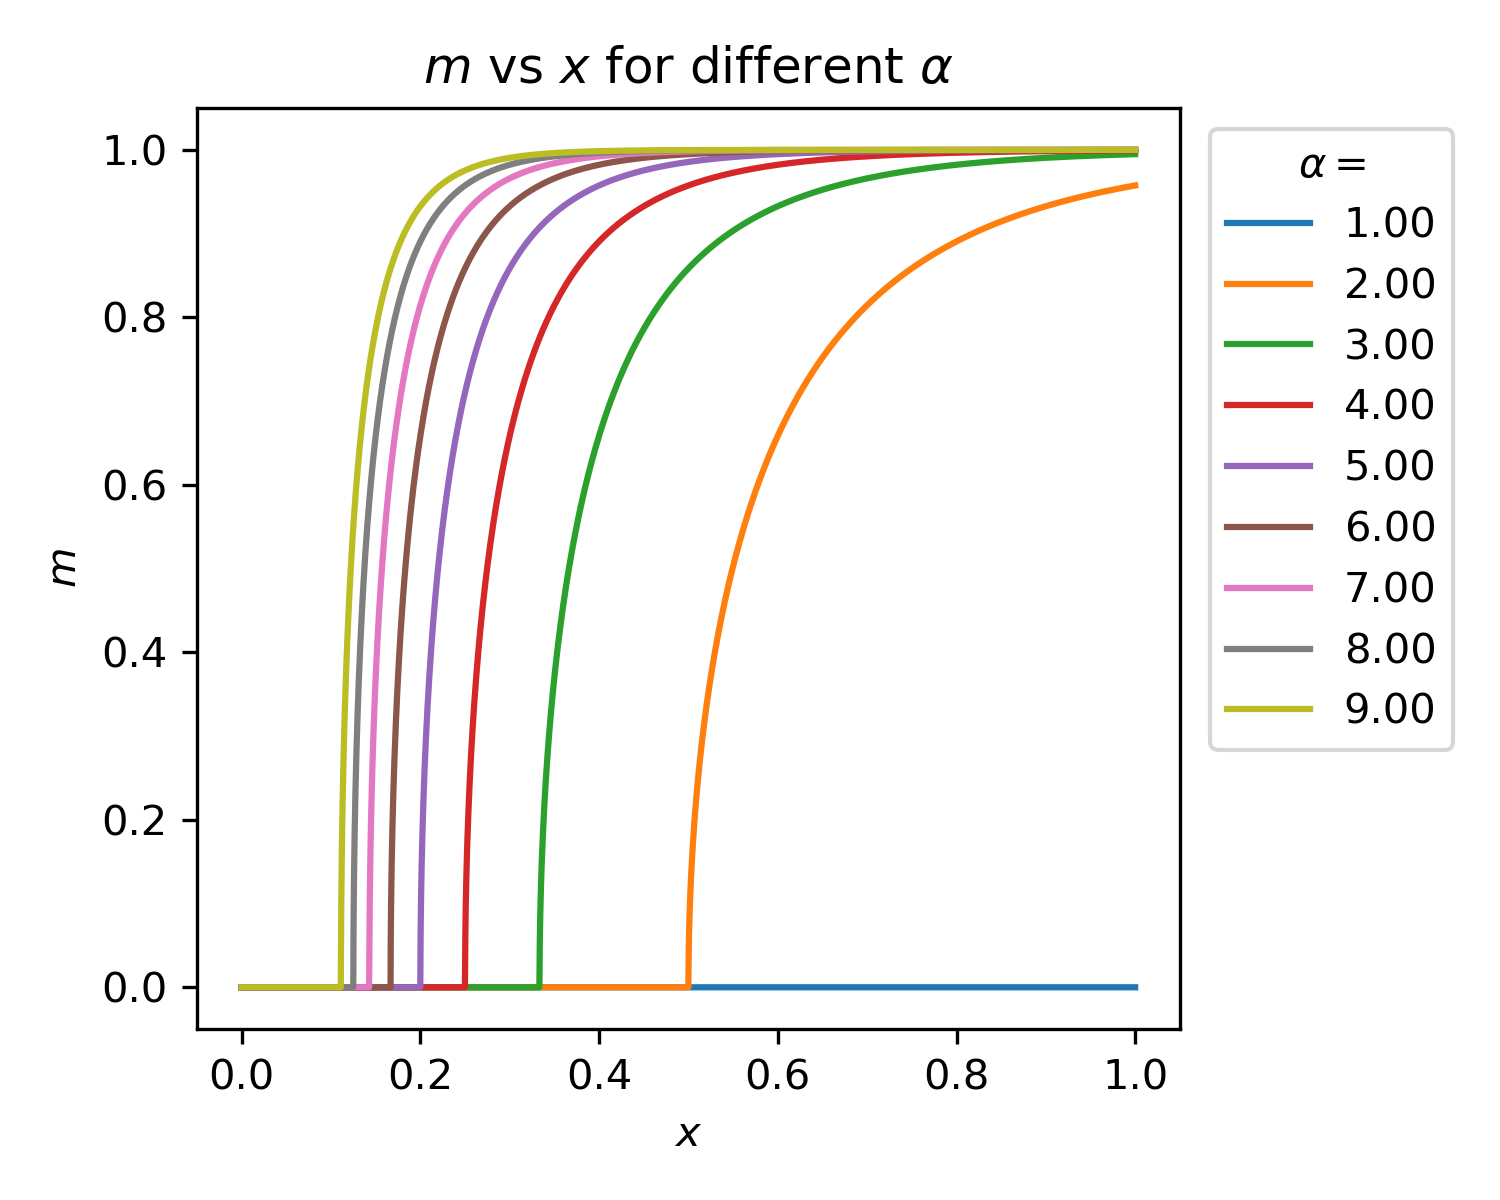
\includegraphics[max width=\textwidth]{m-x.png}
\end{figure}

\subsubsection{}
ii. $g$ vs $\mu$ for $\alpha=\{1,2, \ldots, 9\}$.\\\\
\begin{figure}
  \centering
  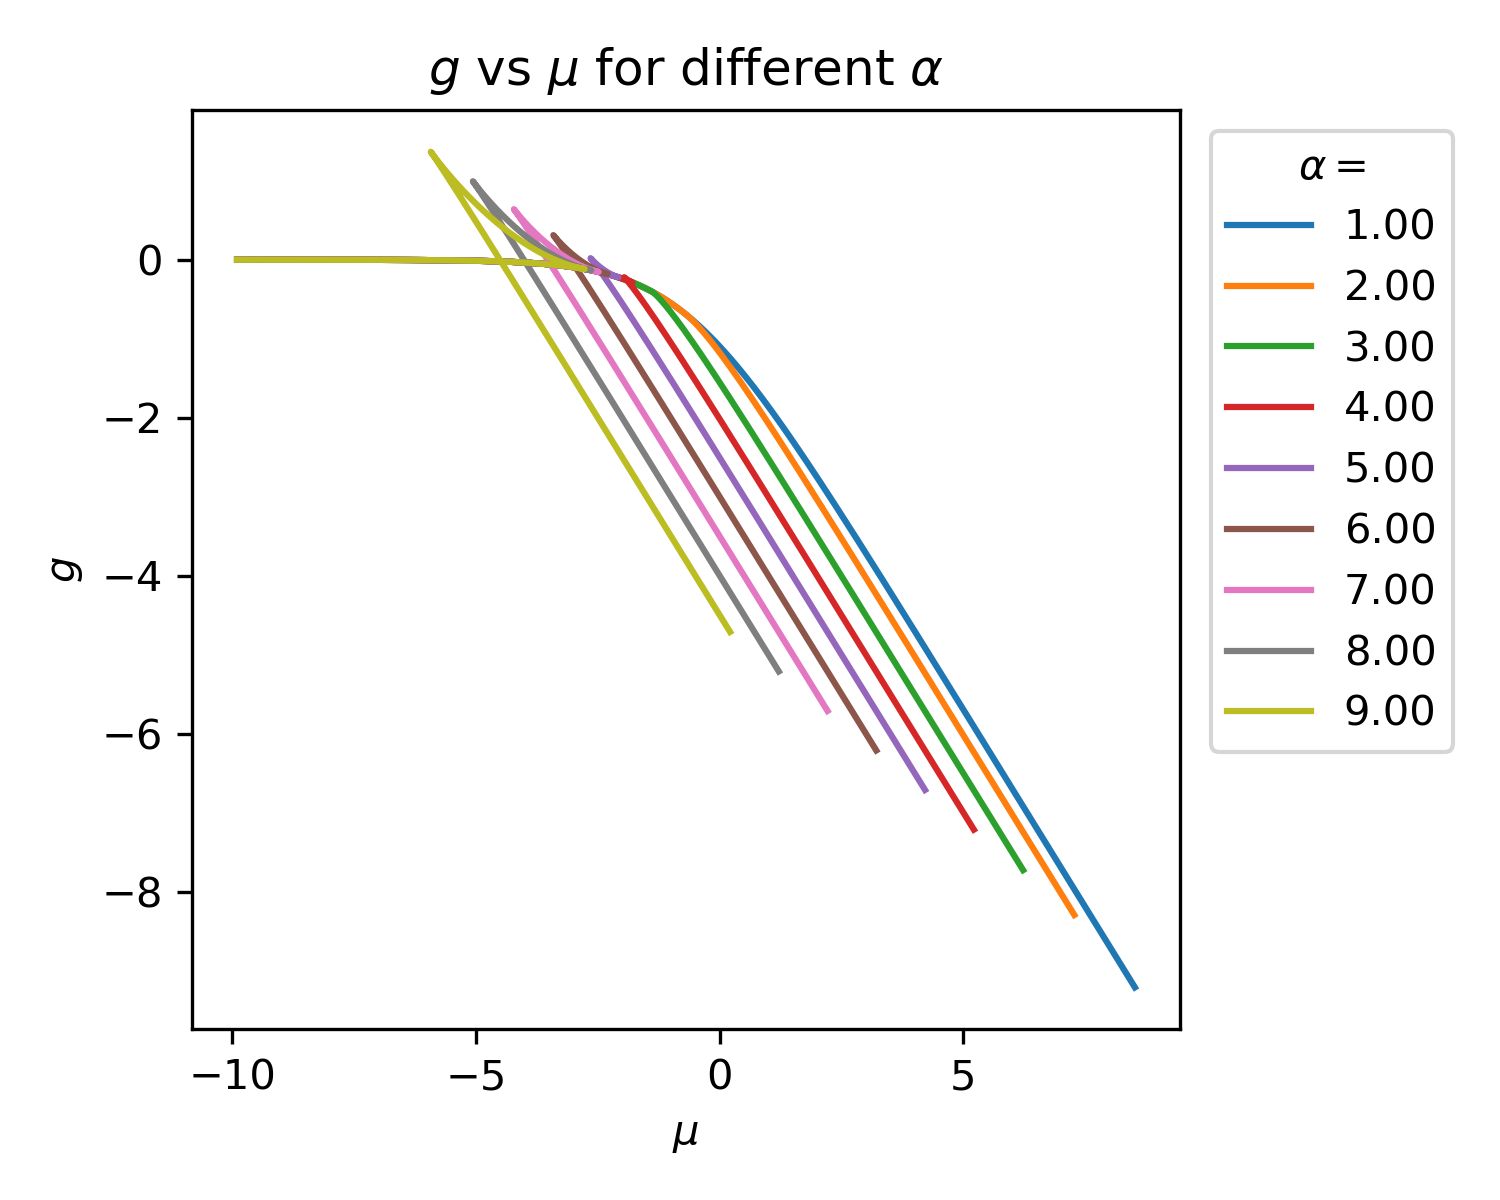
\includegraphics[max width=\textwidth]{g-mu.png}
\end{figure}
iii. For $\alpha=9$, label the following on the $g$ vs $\mu$ plot: (1) stable disordered state, (2) metastable disordered state, (3) stable ordered state, (4) metastable ordered state, (5) unstable state, (6) spinodal of ordered state, (7) spinodal of disordered state, (8) binodal (coexistence).
\newpage
\begin{figure}
  \centering
  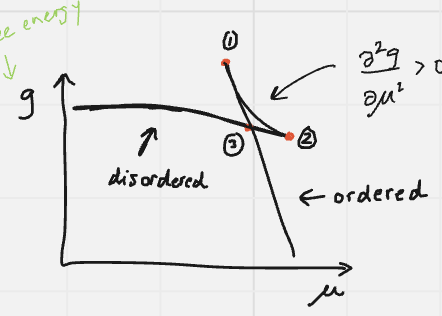
\includegraphics[max width=\textwidth]{drawing.png}
\end{figure}
First of all, we will note that when we have disordered and ordered phases, we have $\frac{\partial ^2 g}{\partial \mu ^2} < 0$, or the curves are concave down. We will start by going along the disordered phase where mu starts at zero. The definition of metastability is when the previously stated thermodynamic condition is met, but the system does not have the lowest free energy. This is clearly the case between the points 2 and 3. At 2, the domain of stability for the disordered phase is reached and the system achieves the spinodal of the disordered phase. In the path between 1 and 2 there is the curve of instability. Now, we will start by considering the curve of the ordered phase. It starts off as stable, until it reaches 3, where it enters a domain of metastability (as discussed earlier) and that goes until 1, which is the spinodal of the ordered phase. In this plot, 3 shows the coexistence of the disordered and ordered phases, which is called the binodal point.
\begin{figure}
  \centering
  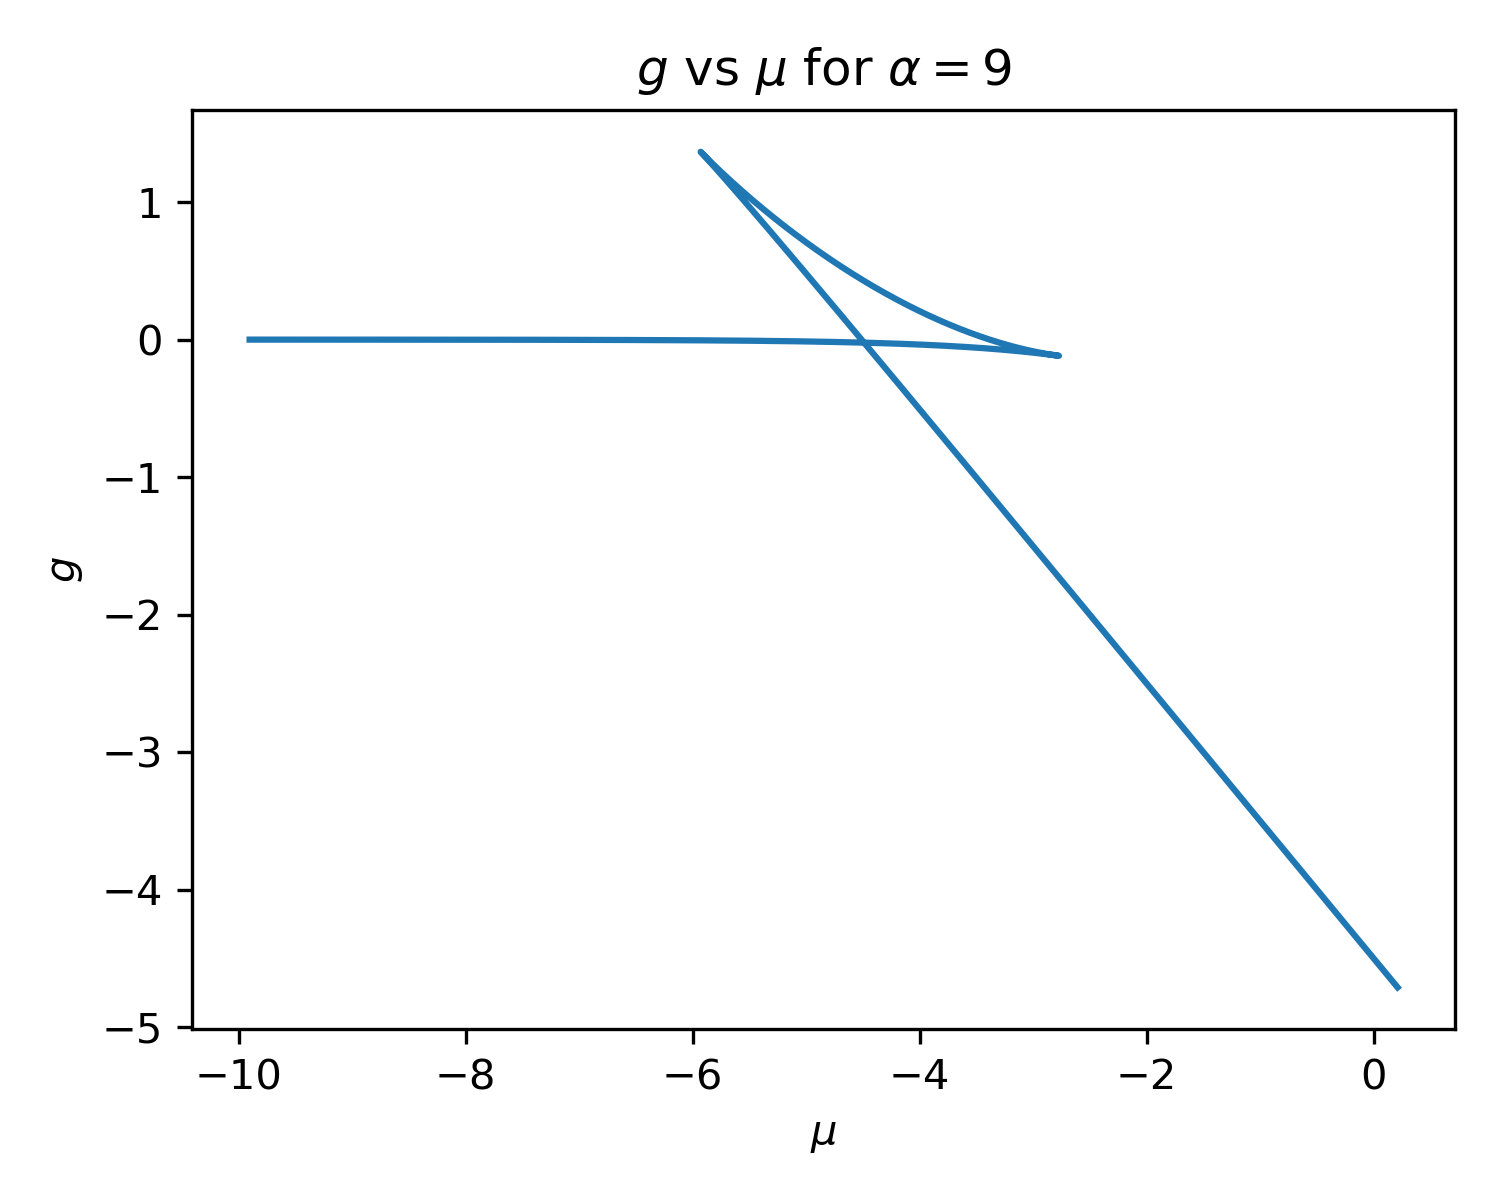
\includegraphics[max width=\textwidth]{g-mu-9.png}  
\end{figure}


iv. Plot the phase diagram in $\alpha-\mu$ space. Use the domains $1 \leq \alpha \leq 9$ and $0<x<1$ to construct the phase diagram. Please use a sufficiently fine grid in each. How does the addition of impurity influence the phase transition? Does this make sense?

Note that above a certain chemical potential, the phase transition will be second order. Below this chemical potential, the phase transition is first order. You will need to obtain the spinodal(s) and binodal in the first order region, and the criticalline or $\lambda$-line in the second order region. The point which joins the two regions is called the tri-critical point.

v. Extra Credit (5 Pts): Plot the phase diagram in $\alpha^{-1}-x_{B}$ space, where $x_{B}=1-x$ is the type B number fraction in the system.
\section{}
\begin{enumerate}
  \setcounter{enumi}{2}
  \item 2-dimensional Monte-Carlo simulation in canonical ensemble
\end{enumerate}

Define a $(40 \times 40)$ square lattice with $N_{A}=x N$ interacting spins that can take $s= \pm 1$ and $N_{B}=N-N_{A}=(1-x) N$ non-interacting spins that can take $s=0$.
\subsection{}
a) Write the Hamiltonian in the canonical ensemble as a function of the spin-state of the system assuming nearest neighbor interactions. Don't forget to account for over counting.\\\\
The Hamiltonian is the same as earlier, but with the exception that here we are just working in the canonical ensemble:
\begin{equation}
  \mathcal{H}=-\frac{1}{2}J \sum_{i=0}^{N_{A}} \sum_{j=0}^{z-1} \tau_{i} \tau_{j}
\end{equation}


b) Write a program to perform Monte Carlo simulations at fixed $(N, x, T)$. For all attempted moves, use the Metropolis-Hastings algorithm to make decisions. Use periodic boundary conditions! Your code should do the following:

i. Start from a random initial state at a given $x$. The interacting spins should be assigned up or down each with probability $1 / 2$.

ii. In each MC iteration, loop over all Type A spins and attempt "flipping" moves.

iii. In each MC iteration, loop over all spins and attempt "swapping" moves with a randomly chosen spin in the immediate vicinity (orthogonally or diagonally touching). Each spin has 4 orthogonally touching spins and 4 spins that are diagonally touching. When attempting a swap, randomly choose 1 out of these 8 possibilities.

iv. Plot the total energy $E$ vs iteration number $i$.

v. Plot the relative magnetization $m$ vs iteration number $i$.

vi. Print a visual snapshot of both the initial and final configurations. (in MATLAB, for a matrix $\mathrm{A}$, imagesc(A) will display the matrix as an image).\\
% Inline Python code in the document
\begin{lstlisting}[language=Python]
import numpy as np
import matplotlib.pyplot as plt
from matplotlib import colors
import random

class MonteCarlo():

    def __init__(self, x, alpha, n_iter):
        self.x = x  # Fraction of interacting spins
        self.beta = alpha  # Inverse temperature
        self.ni = int(n_iter)  # Number of iterations
        self.N = 1600
        self.ndim = int(np.sqrt(self.N))  # Assuming a square lattice
        self.Na = int(self.N*x)
        self.Nb = int(self.N - self.Na)

        np.random.seed(24)

        # Initialize a two-dimensional square lattice
        state = np.zeros((self.ndim, self.ndim), dtype=int)

        # Randomly choose Na positions in the lattice for the interacting spins
        interacting_indices = np.random.choice(self.N, self.Na, replace=False)

        # Convert linear indices to 2D indices and assign s = +/- 1 to these positions
        for index in interacting_indices:
            i, j = divmod(index, self.ndim)
            state[i, j] = np.random.choice([-1, 1])
 


        
   
        self.oldstate = np.copy(state)
        self.newstate = np.copy(state)

        self.initial = np.copy(state)
        self.E = 0
        for i in range(40):
            for j in range(40):
                self.E += self.local_hamiltonian(i, j, self.oldstate)
        self.E /= 2 #overcounting
        self.dE = 0 #placeholder

    def plot_state(self, state, n_iter, title="Lattice State"):
        plt.figure(figsize=(6, 6))
        plt.title(title)
        plt.imshow(state, cmap='viridis', interpolation='nearest')
        plt.colorbar(label='Spin Value')
        # Dynamically generate the filename using the iteration number
        filename = f"lattice_state_{n_iter}_{self.x}.png"
        plt.savefig(filename)
        plt.close()  # Close the figure after saving to free up memory
        return
        


    
    def run_iter(self):
        # first consider the flips
        for i in range(self.ndim):
            for j in range(self.ndim):
                # consider all possible flips only for the interacting spins
                if abs(self.oldstate[i][j]) == 1:
                    self.flip(i, j)
                    # calculate the change in energy associated
                    self.dE = self.local_hamiltonian(i, j, self.newstate) - self.local_hamiltonian(i, j, self.oldstate)
                    self.dE *= self.beta
                    # except or reject the switch based off of the metropolis-hastings algorithm
                    if self.update():
                        self.accept()
                    self.newstate = np.copy(self.oldstate)
                    
        # now consider the swaps
        for i in range(self.ndim):
            for j in range(self.ndim):
                # no need to check whether the spins are interacting or not
                neighbor = self.swap(i, j)
                # calculate the change new energy associated
                new_energy = self.local_hamiltonian(i, j, self.newstate) + self.local_hamiltonian(neighbor[0], neighbor[1], self.newstate)
                old_energy = self.local_hamiltonian(i, j, self.oldstate) + self.local_hamiltonian(neighbor[0], neighbor[1], self.oldstate)
                self.dE = new_energy - old_energy
                self.dE *= self.beta
                # except or reject the switch based off of the metropolis-hastings algorithm
                if self.update():
                    self.accept()
                self.newstate = np.copy(self.oldstate)       
        return

        
                

            
    
    def flip(self, i, j):
        ################################################################
        # THIS FUNCTION SHOULD PERFORM A FLIP AT INDEX i AND j, AND    #
        # COMPUTE THE ASSOCIATED ENERGY CHANGE WITH THiS FLIP          #
        ################################################################
        # changed the sign at index i, j
        self.newstate[i][j] = -self.newstate[i][j]
        return



    def swap(self, i, j):
        ################################################################
        # THIS FUNCTION SHOULD PERFORM A SWAP OF INDEX i AND j, AND    #
        # COMPUTE THE ASSOCIATED ENERGY CHANGE WITH THiS SWAP          #
        ################################################################
        # Define offsets for the 8 neighbors: top, bottom, left, right, and the 4 diagonals
        offsets = [(-1, 0), (1, 0), (0, -1), (0, 1), (-1, -1), (-1, 1), (1, -1), (1, 1)]
        # compute their indices given the periodic boundary conditions, which means taking mod self.ndim
        neighbors = [((i + di) % self.ndim, (j + dj) % self.ndim) for di, dj in offsets]
        # choose a random neighbor using random.choice
        neighbor = random.choice(neighbors)
        # swap the spins
        self.newstate[i][j], self.newstate[neighbor[0]][neighbor[1]] = self.newstate[neighbor[0]][neighbor[1]], self.newstate[i][j]
        # returned the index of the neighbor that was chosen
        return neighbor


    
    def update(self):

        ################################################################
        # THIS FUNCTION SHOULD CHECK WHETHER OR NOT A GIVEN OPERATION  #
        # SHOULD BE ACCEPTED. THIS IS YOUR METRPOLIS-HASTING ALGORITHM #
        ################################################################
        
        condition = False
        if self.dE <= 0 or np.random.rand() <= np.exp(-self.dE):
            condition = True
        # REGARDLESS OF THE OUTCOME ABOVE, YOU STILL NEED TO INITILIASE
        # YOUR NEW STATE FOR THE NEXT ITERATION
        # self.newstate = np.copy(self.oldstate)
        return condition
        


    def accept(self):
        ################################################################
        # THIS FUNCTION SHOULD UPDATE YOUR OLDSTATE AND ENERGY GIVEN   #
        # A CHANGE WAS ACCEPTED                                        $
        ################################################################
        self.oldstate = np.copy(self.newstate)
        self.E += self.dE
        return


    
    def local_hamiltonian(self, i, j, state):
        E = 0
        ################################################################
        # THIS FUNCTION SHOULD CALCULATE THE CHANGE IN THE HAMILTONIAN #
        # LOCALLY AROUND i and j. REMEMBER TO ACCOUNT FOR PERIOD BOUN- #
        # -DARY CONDITIONS.                                            #
        ################################################################
        # we only add a contribution to the energy if the spin is interacting
        if abs(state[i][j]) == 1:
            # Define offsets for the 4 neighbors: top, bottom, left, right, 
            offsets = [(-1, 0), (1, 0), (0, -1), (0, 1)]
            # compute their indices given the periodic boundary conditions, which means taking mod self.ndim
            neighbors = [((i + di) % self.ndim, (j + dj) % self.ndim) for di, dj in offsets]
            # check if the neighbor is in interacting spin
            for neighbor in neighbors:
                if abs(state[neighbor[0]][neighbor[1]]) == 1:
                    E += -state[i][j] * state[neighbor[0]][neighbor[1]]       
        return E
    

    def get_energy(self):
        return self.E

    def get_m(self):
        ################################################################
        # THiS FUNCTION SHOULD CALCULATE THE AVERAGE MAGNETISATION OF  #
        # YOUR SYSTEM AT A GIVEN ITERATION.                            #
        ################################################################
        magnetization = (1/self.Na) * np.sum(self.oldstate)
        return magnetization
    
    def run(self):
        self.initial = np.copy(self.oldstate)

        self.ms = [self.get_m()]
        self.Es = [self.get_energy()]

        for i in range(self.ni):
            # plot the state if it is the initial state
            if i == 0:
                self.plot_state(self.oldstate, i, title='Initial Lattice State')

            self.run_iter()

            
            self.Es.append(self.get_energy())
            self.ms.append(self.get_m())
            # plot the state if it is the final state
            if i == self.ni - 1:
                self.plot_state(self.oldstate, i, title='Final Lattice State')
                
        
        self.final = self.oldstate
def plot_magnetization_vs_iterations(x, alpha, n_iter):
    plt.figure()
    plt.plot(MC.ms)
    plt.xlabel('Iterations')
    plt.ylabel('Magnetization')
    plt.title(f'Magnetization vs Iterations for x = {x}')
    plt.savefig(f'magnetization_vs_iterations_{x}.png')
    return
def plot_energy_vs_iterations(x, alpha, n_iter):
    plt.figure()
    plt.plot(MC.Es)
    plt.xlabel('Iterations')
    plt.ylabel('Energy')
    plt.title(f'Energy vs Iterations for x = {x}')
    plt.savefig(f'energy_vs_iterations_{x}.png')
    return

x = [1, 0.75, 0.4]
alpha = [0.5, 3, 1]
n_iters = [1e3, 1e4, 1e4]

# make a dictionary for all of the trials whose entries are given in the correct order in the lists above
trials = {'x': x, 'alpha': alpha, 'n_iters': n_iters}
for i in range(3):
    MC = MonteCarlo(trials['x'][i], trials['alpha'][i], trials['n_iters'][i])
    MC.run()
    # plot the energies vs the number of iterations
    plot_energy_vs_iterations(trials['x'][i], trials['alpha'][i], trials['n_iters'][i])
    # plot the magnetization vs the number of iterations
    plot_magnetization_vs_iterations(trials['x'][i], trials['alpha'][i], trials['n_iters'][i])



# print(MC.initial)

# print(MC.final)
# print(MC.ms)
# plot the energies vs the number of iterations


\end{lstlisting}

c) Run the following simulations. For each simulation provide the following: (1) $E$ vs $i$ plot, (2) $m$ vs $i$ plot, (3) snapshots of the initial and final configurations.\\
\emph{I will show the plots for the simulations in the order that is given.}
\newpage
i. $x=1, J / k T=0.5, n_{\text {iters }}=10^{3}$.\\
\begin{figure}
  \centering
  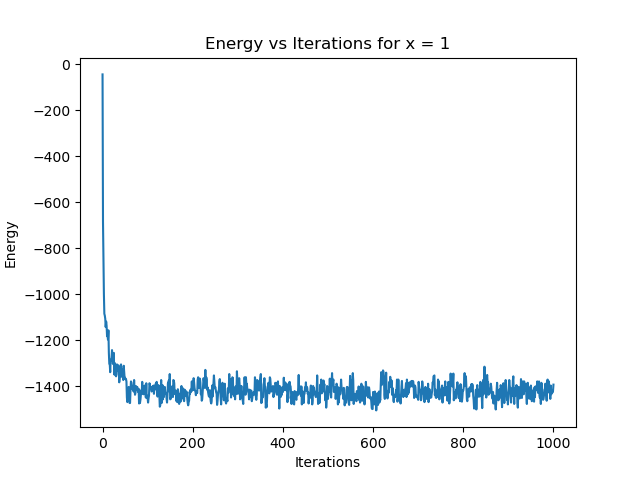
\includegraphics[max width=\textwidth]{energy_vs_iterations_1.png}
\end{figure}
\begin{figure}
  \centering
  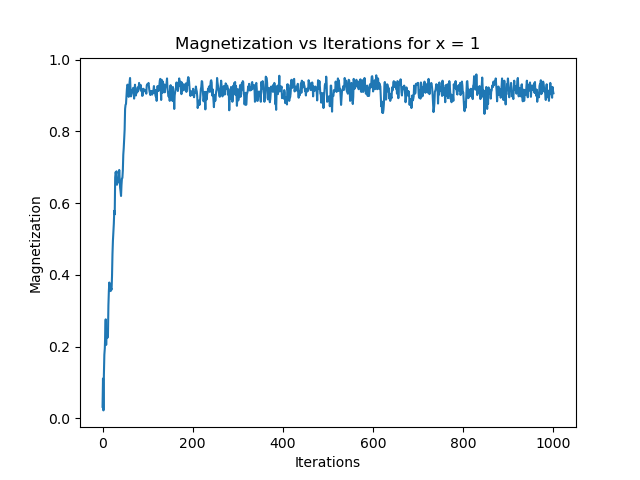
\includegraphics[max width=\textwidth]{magnetization_vs_iterations_1.png}
\end{figure}
\begin{figure}
  \centering
  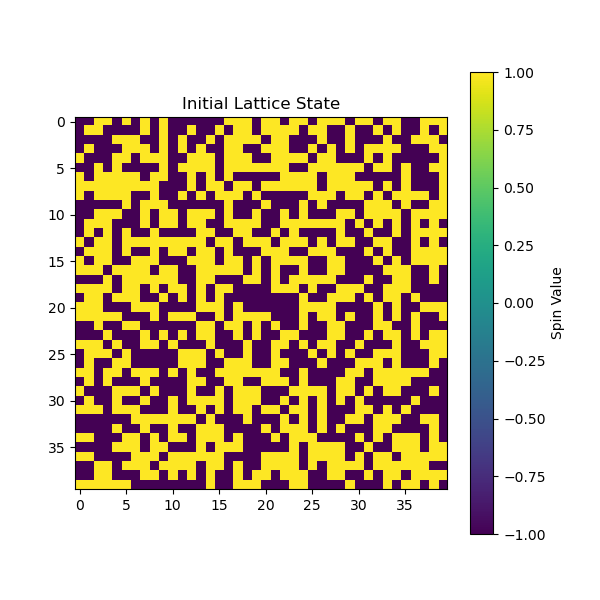
\includegraphics[max width=\textwidth]{lattice_state_0_1.png}
\end{figure}
\begin{figure}
  \centering
  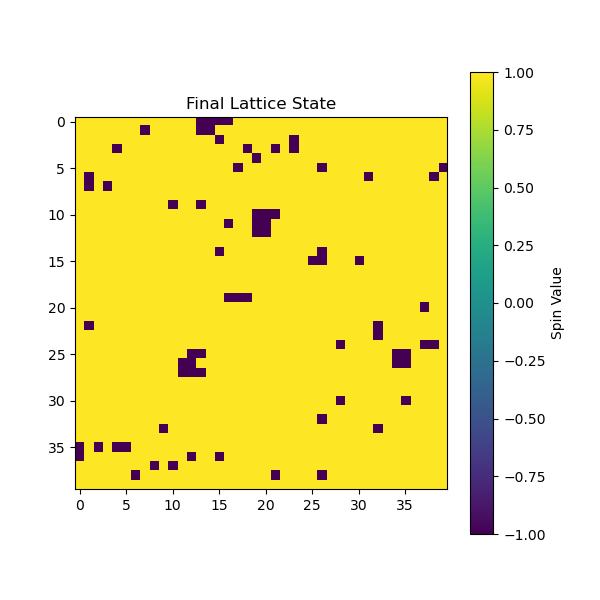
\includegraphics[max width=\textwidth]{lattice_state_999_1.png}
\end{figure}
\newpage

ii. $x=0.75, J / k T=3, n_{\text {iters }}=10^{4}$.\\
\begin{figure}
  \centering
  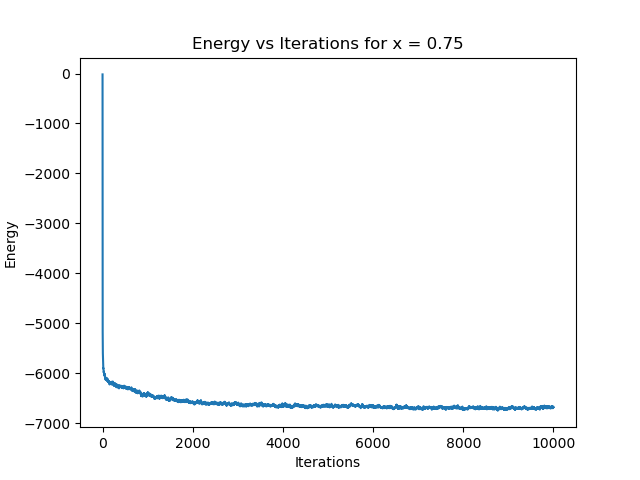
\includegraphics[max width=\textwidth]{energy_vs_iterations_0.75.png}
\end{figure}
\begin{figure}
  \centering
  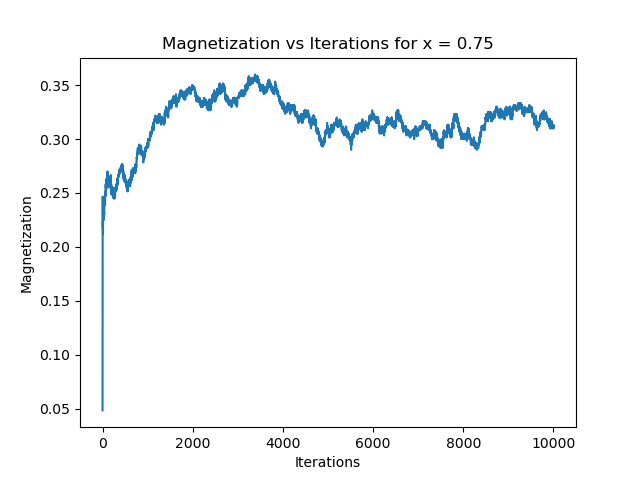
\includegraphics[max width=\textwidth]{magnetization_vs_iterations_0.75.png}
\end{figure}
\begin{figure}
  \centering
  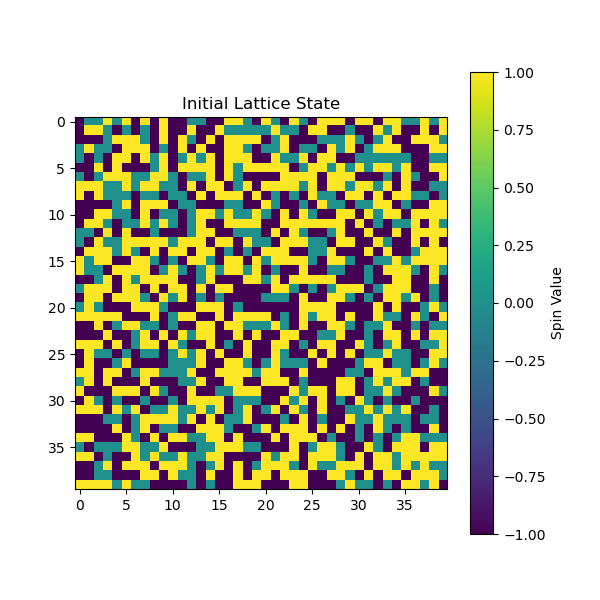
\includegraphics[max width=\textwidth]{lattice_state_0_0.75.png}
\end{figure}
\begin{figure}
  \centering
  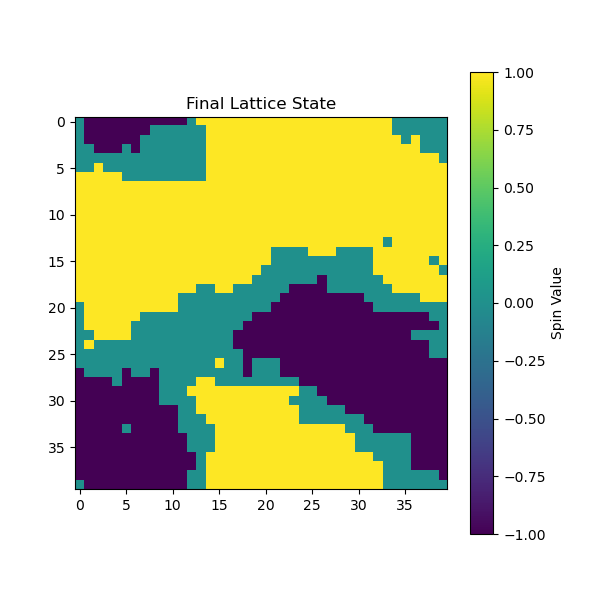
\includegraphics[max width=\textwidth]{lattice_state_9999_0.75.png}
\end{figure}
\newpage
\begin{figure}
  \centering
  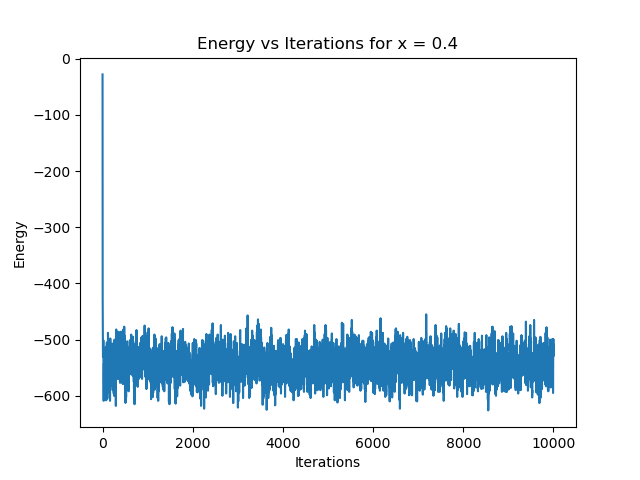
\includegraphics[max width=\textwidth]{energy_vs_iterations_0.4.png}
\end{figure}
\begin{figure}
  \centering
  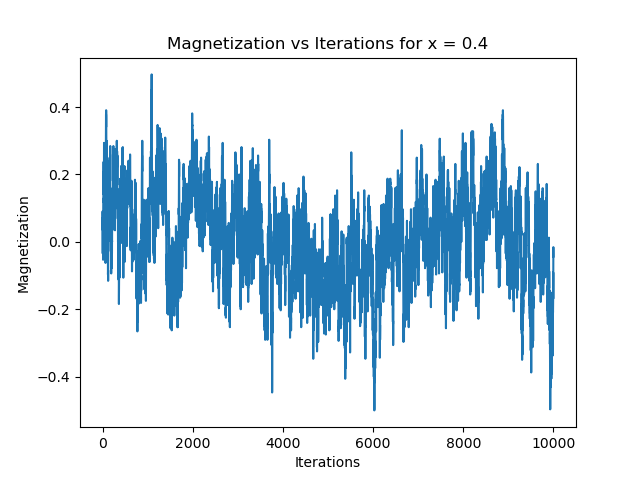
\includegraphics[max width=\textwidth]{magnetization_vs_iterations_0.4.png}
\end{figure}
\begin{figure}
  \centering
  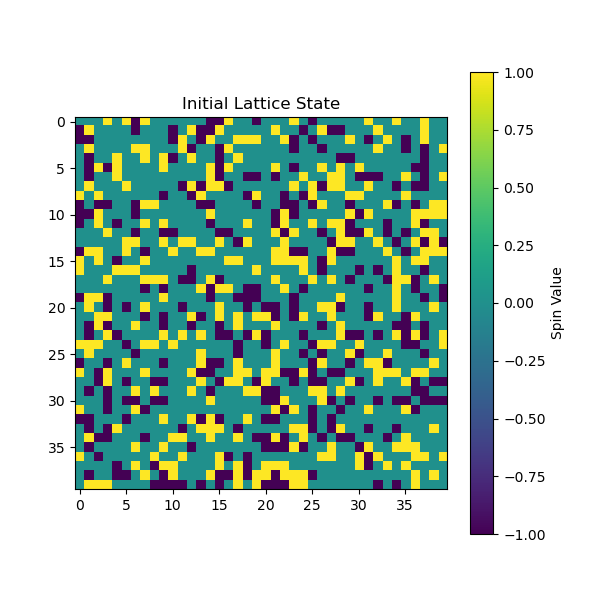
\includegraphics[max width=\textwidth]{lattice_state_0_0.4.png}
\end{figure}
\begin{figure}
  \centering
  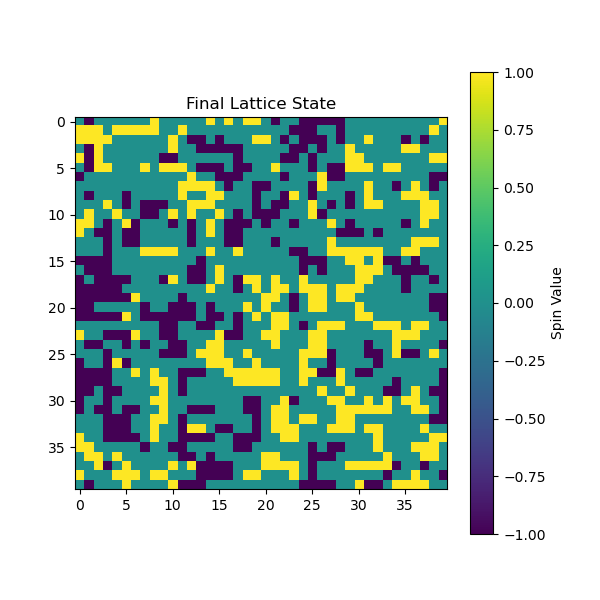
\includegraphics[max width=\textwidth]{lattice_state_9999_0.4.png}
\end{figure}

iii. $x=0.4, J / k T=1, n_{\text {iters }}=10^{4}$.
\newpage

d) Extra Credit ( 8 pts): Plot $m$ vs $x$ for $J / k T=1$. You should use $n_{\text {iters }} \geq 10^{4}$ for the best results. You will need to average over the trajectory once equilibrium is reached to get an $\langle m\rangle$ for each $x$.

\begin{figure}
  \centering
  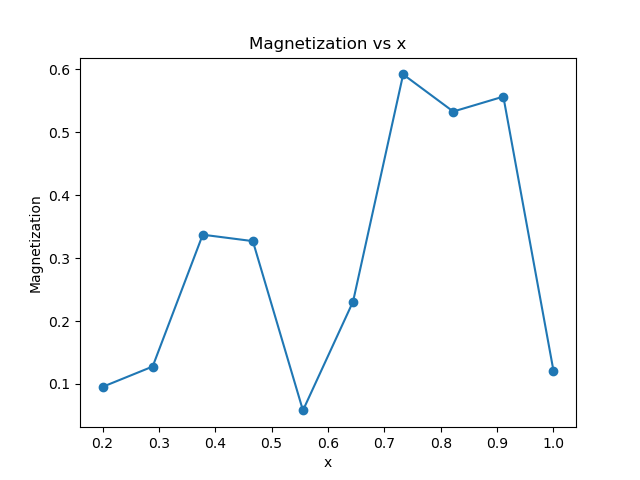
\includegraphics[max width=\textwidth]{magnetization_vs_x.png}
\end{figure}
% Inline Python code in the document
\begin{lstlisting}[language=Python]
# Define parameters
x = np.linspace(0.2, 1, 10)
alpha = 3
n_iters = int(1e4)  # Ensure n_iters is an integer

# Initialize an empty list for plotting
x_m = []

# Loop over different values of x
for i in range(len(x)):
    MC = MonteCarlo(x[i], alpha, n_iters)
    MC.run()
    # Get the absolute value of the average value of the magnetization over the last 500 iterations
    m = np.mean(np.abs(MC.ms[500:]))
    # Store the value in a tuple like (x, m)
    x_m.append((x[i], m))

# Extract x and m values for plotting
x_values, m_values = zip(*x_m)

# Plot the information
plt.figure()
plt.plot(x_values, m_values, marker='o')  # Added marker for clarity
plt.xlabel('x')
plt.ylabel('Magnetization')
plt.title('Magnetization vs x')
plt.savefig('magnetization_vs_x_2.png')
\end{lstlisting}

\end{document}